\documentclass[12pt]{beamer}

\geometry{paperwidth=140mm,paperheight=105mm}

\usepackage{../fenna-files/packages-presentation}
\addbibresource{../fenna-files/references.bib}
\usepackage{../fenna-files/abbreviations}

\usepackage{framed} %boxes
\newcommand*{\mybox}[1]{\framebox{#1}} %box around word

\usepackage{booktabs}

\usepackage{graphicx}

% \def\bibfont{\tiny}

% \usepackage{fixltx2e}

% Choose how your presentation looks.
%
% For more themes, color themes and font themes, see:
% http://deic.uab.es/~iblanes/beamer_gallery/index_by_theme.html
%
\mode<presentation>
{
\usetheme{Madrid}      % or try Darmstadt, Madrid, Warsaw, ...
\definecolor{goethe}{rgb}{0,0.37,0.66}
\usecolortheme[named=goethe]{structure}
	% \usefonttheme{serif}  % or try serif, structurebold, ...
\setbeamertemplate{navigation symbols}{}
\setbeamertemplate{caption}[numbered]
\resetcounteronoverlays{exx}
}

\renewcommand{\eachwordone}{\sffamily}
\renewcommand{\eachwordtwo}{\sffamily}
\renewcommand{\eachwordthree}{\sffamily}

%gets rid of bottom navigation bars
\setbeamertemplate{footline}{}

%gets rid of navigation symbols
%\setbeamertemplate{navigation symbols}{}


\addtobeamertemplate{navigation symbols}{}{%
\usebeamerfont{footline}%
\usebeamercolor[fg]{footline}%
\hspace{1em}%
\insertframenumber/\inserttotalframenumber
}


\title{Case competition in headless relatives: a Germanic typology}
\author{Fenna Bergsma}
\institute{\normalsize Goethe-Universität Frankfurt}
\date{GK colloquium\\ \today}


\begin{document}


\begin{frame}
\titlepage

\centering{

\includegraphics[width=0.4\textwidth]{dfg-logo}
\hspace{2cm}

\includegraphics[width=0.3\textwidth]{goethe-logo}}
\end{frame}

\begin{frame}{Case competition in headless relatives}

  \pause

\begin{itemize}
  \item \tbf{case competition}: a situation in which two cases are assigned but only one of them surfaces \pause
  \item \tbf{headless relative}: a relative clause construction that lacks a head \pause
\end{itemize}

\vspace{1em}

\exg. Ich {lade ein} \mybox{\tbf{wem}} \tbf{auch} \tbf{Maria} \tbf{vertraut}. \\
 I invite\scsub{[acc]} \ac{rel}.\ac{dat}.\tsc{an} also Maria trusts\scsub{[dat]}.\\
 `I invite whoever Maria also trusts.' \flushfill{Modern German, \pgcitealt{vogel2001}{344}}\label{ex:mg-acc-dat-intro}

\end{frame}

%

\begin{frame}{The content of my dissertation}

\pause

\begin{itemize}
  \item headless relatives in three Germanic languages:
  \begin{itemize}
    \item Gothic
    \item Old High German
    \item Modern German
  \end{itemize}\pause
  \item two aspects:
  \begin{itemize}
    \item one is stable crosslinguistically
    \item one differs crosslinguitically
  \end{itemize}
\end{itemize}

\end{frame}
%%

\begin{frame}{The crosslinguistically stable one}

\pause

\ex. \ac{nom} < \ac{acc} < \ac{dat}\pause

\exg. Ich {lade ein} \mybox{\tbf{wem}} \tbf{auch} \tbf{Maria} \tbf{vertraut}. \\
 I invite\scsub{[acc]} \ac{rel}.\ac{dat}.\tsc{an} also Maria trusts\scsub{[dat]}.\\
 `I invite whoever Maria also trusts.' \flushfill{Modern German, \pgcitealt{vogel2001}{344}}\label{ex:mg-acc-dat-rep} \pause

this case scale is not unique to case competition in headless relatives \pause

\begin{itemize}
  \item in syntax
  \begin{itemize}
    \item agreement \citep[cf.][]{moravcsik1978}
    \item relativization \citep[cf.][]{keenan1977}
  \end{itemize} \pause
  \item in morphology
  \begin{itemize}
    \item syncretism patterns \citep[cf.][]{baerman2005}
    \item formal containment \citep[cf.][]{caha2010}
  \end{itemize}
\end{itemize}


\end{frame}
%%

\begin{frame}{A reflex of morphology in syntax}

\pause

\citealt[cf.][]{caha2009}

\begin{table}[h]
  \center
		\begin{tabular}[b]{cc}
      \begin{forest} boom
      [\tsc{dat}P,name=datp
          [\tsc{dat},name=dat]
          [\ac{acc}P,name=accp,
          tikz={
          \node[draw,circle,
          xscale=0.75,yscale=0.95,
          color=white,
          fit=(accp)(acc)(x)]{};
          }
              [\ac{acc},name=acc],
              tikz={
              \node[draw,circle,
              xscale=0.75,yscale=0.95,
              color=white,
              fit=(nomp)(nom)(x)]{};
              }
              [\tsc{nomP},name=nomp
                  [\ac{nom},name=nom]
                  [NP,name=np
                      [...,name=x,
                      roof,baseline
                      ]
                  ]
              ]
          ]
      ]
      \end{forest}
      &\pause
      \begin{forest} boom
    [\tsc{acc}P,name=accp
        [\tsc{acc},name=acc],
        tikz={
        \node[draw,circle,
        xscale=0.75,yscale=0.95,
        color=white,
        fit=(accp)(acc)(x)]{};
        }
        [{\tsc{nomP}},name=nomp
            [{\ac{nom}},name=nom]
            [NP,name=np
                [...,name=x,
                roof,baseline
                ]
            ]
        ]
    ]
      \end{forest}\\
  \end{tabular}
\end{table}


\end{frame}


\begin{frame}{A reflex of morphology in syntax}

\citealt[cf.][]{caha2009}

  \begin{table}[H]
    \center
  	% \caption {\ac{dat}P deletes \ac{acc}P}
  		\begin{tabular}[b]{c c}
        \begin{forest} boom
          [\tsc{datP}
              [\ac{dat}]
                [\ac{acc}P,name=accp,
                tikz={
                \node[draw,circle,
                xscale=0.775,yscale=0.975,
                fit=(accp)(acc)(nom)(x)]{};
                }
                  [\ac{acc},name=acc]
                  [\tsc{nomP},name=nomp
                      [\ac{nom},name=nom]
                      [NP,name=np
                          [...,name=x, roof ,baseline]
                      ]
                  ]
              ]
          ]
        \end{forest}
        &
        \begin{forest} boom
          [\textcolor{LG}{\tsc{accP}},name=accp,
          tikz={
          \node[draw,circle,
          xscale=0.775,yscale=0.975,
          fit=(accp)(acc)(nom)(x)]{};
          }
              [\textcolor{LG}{\ac{acc}},name=acc,edge=LG]
              [\textcolor{LG}{\tsc{nomP}},name=nomp,edge=LG
                  [\textcolor{LG}{\ac{nom}},name=nom,edge=LG]
                  [\textcolor{LG}{NP},name=np,edge=LG
                      [\textcolor{LG}{...},name=x,
                      roof, baseline, edge=LG
                      ]
                  ]
              ]
          ]
        \end{forest} \\
    \end{tabular}
  \end{table}

\end{frame}

%%

\begin{frame}{The crosslinguistically differing one}

\pause

\begin{itemize}
  \item \tbf{internal case} refers to the case associated with the relative pronoun internal to the relative clause
  \item \tbf{external case} refers to the case associated with the missing head in the main clause, which is external to the relative clause
\end{itemize}

\pause

\begin{table}[h]
	\center
		\begin{tabular}{ccc}
		\toprule
		 					      & \ac{int}>\ac{ext}		& \ac{ext}>\ac{int}	\\
								      \cmidrule{2-3}
		Gothic		      &	\tsc{int}						&	\tsc{ext}					\\
		Modern German 	& \tsc{int}						&	*			  					\\
		Old High German	& *								   	&	\tsc{ext}					\\
		\bottomrule
		\end{tabular}
\end{table}

\end{frame}

%%

\begin{frame}{Gothic: both}

\exg. ushafjands \tbf{ana} \mybox{\tbf{þamm}} \tbf{-ei} \tbf{lag}\\
{picking up}\scsub{[acc]} on\scsub{[dat]} \ac{rel}.\ac{dat}.\ac{n}.\ac{sg} -\ac{comp} lay\\
`picking up (that) on which he lay' \flushfill{Gothic, \ac{luke} 5:25, adapted from \pgcitealt{harbert1978}{343}}\label{ex:gothic-acc-dat-rep}

\exg. hva nu wilei ei taujau \mybox{þamm} \tbf{-ei} \tbf{qiþiþ} \tbf{þiudan} \tbf{Iudaie}?\\
 what now want that do\scsub{[dat]} \ac{rel}.\ac{dat}.\ac{m}.\ac{sg} -\ac{comp} say\scsub{[acc]} king {of Jews}\\
 `what now do you wish that I do to (him) whom you call King of the Jews?' \flushfill{Gothic, \ac{mark} 15:12, adapted from \pgcitealt{harbert1978}{339}}\label{ex:gothic-dat-acc-rep}

\end{frame}

%%

\begin{frame}{Modern German: only internal}

\exg. Ich {lade ein} \mybox{\tbf{wem}} \tbf{auch} \tbf{Maria} \tbf{vertraut}. \\
 I invite\scsub{[acc]} \ac{rel}.\ac{dat}.\tsc{an} also Maria trusts\scsub{[dat]}.\\
 `I invite whoever Maria also trusts.' \flushfill{Modern German, \pgcitealt{vogel2001}{344}}\label{ex:mg-acc-dat}

\exg. *Ich vertraue \mybox{wem} \tbf{auch} \tbf{Maria} \tbf{mag}. \\
I trust\scsub{[dat]} \ac{rel}.\ac{dat}.\tsc{an} also Maria likes\scsub{[acc]}.\\
`I trust whoever Maria also likes.' \flushfill{Modern German, \pgcitealt{vogel2001}{345}}

\end{frame}

%%

\begin{frame}{Old High German: only external}

\exg. bistû furira Abrâhame, ouh \mybox{thên} \tbf{man} \tbf{hiar} \tbf{nû} \tbf{zalta}?\\
 {are you} older\scsub{[dat]} {to Abraham} also \ac{rel}.\ac{dat}.\tsc{pl} one here now named\scsub{[acc]}\\
 `are you really older than Abraham and those who have been mentioned here?' \flushfill{Old High German, \ac{otfrid} III 18:33, \pgcitealt{behaghel1923}{761}}\label{ex:ohg-dat-acc}

\end{frame}

%%


\begin{frame}{Different patterns and different pronouns?}

  \begin{table}[h]
  	\center
  		\begin{tabular}{cccc}
  		\toprule
                      & \multicolumn{2}{l}{headless relatives}  & \only<2-3>{relative pronoun}    \\
  		 					      & \ac{int}>\ac{ext}		& \ac{ext}>\ac{int}	&                                \\
  								      \cmidrule{2-3}
  		Gothic		      &	\tsc{int}						&	\tsc{ext}					& \only<2-3>{\tsc{d} + ϕ + \tsc{comp}} \\
  		Modern German 	& \tsc{int}			 			&	*								  & \only<2-3>{\tsc{wh} + ϕ}             \\
  		Old High German	& * 									&	\tsc{ext}			   	& \only<2-3>{\tsc{d} + ϕ}              \\
  		\bottomrule
  		\end{tabular}
  \end{table}

\vspace{2em}

\pause\pause

\centering{
how?
}

\end{frame}

%%

\begin{frame}{\posscitet{cinqueforthcoming} double-headed analysis}

	\begin{minipage}[t]{0.47\textwidth}
  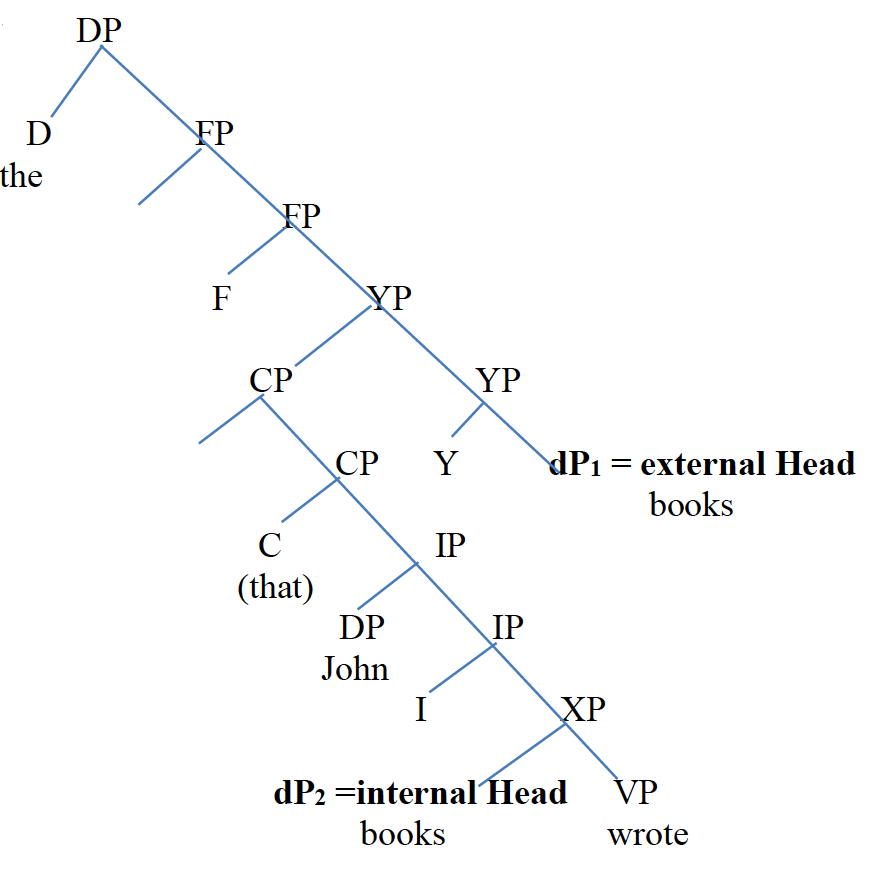
\includegraphics[width=1.1\linewidth]{cinque-tree}    \pause

  \end{minipage}\hfill\vline\hfill
	\begin{minipage}[t]{0.47\textwidth}
    \vspace{-15em}
\begin{itemize}
  \item raising analysis
  \begin{itemize}
    \item \tit{Had he continued to be dean, he could not have written the books that he wrote.}
    \item dP₂ moves to specCP and deletes dP₁
    \item amount interpretation
  \end{itemize} \pause
  \item matching analysis
  \begin{itemize}
    \item \tit{The book that John wrote lies on the shelf.}
    \item dP₁ moves to specFP and deletes dP₂
    \item individual interpretation
  \end{itemize}
\end{itemize}

	\end{minipage}

\end{frame}


\begin{frame}{The variation explained in a nutshell}

  \begin{itemize}
    \item the relative pronoun in Old High German is actually the \tbf{external head} which has deleted the (attracted) relative pronoun
    \item in Modern German, the relative pronoun in the relative clause deletes an \tbf{indefinite}
    \item Gothic: ?
  \end{itemize}

\end{frame}


\begin{frame}{Old High German: attraction in headed relatives}

\pause

\exg. unde ne wolden níet besên \textcolor{goethe}{den} \textcolor{goethe}{mort} \mybox{\tbf{\textcolor{goethe}{den}}} \tbf{dô} \tbf{was} \tbf{geschên}\\
 and not wanted not see\scsub{[acc]} the.\tbf{\ac{acc}}.\ac{sg} murder \ac{rel}.\tbf{\ac{acc}}.\ac{sg} there had happened\scsub{[nom]}\\
 `and they didn't want to see the murder that had happened.' \flushfill{Middle High Germans, \ac{nib} 1391,14, \pgcitealt{grimm1866}{319}, after \pgcitealt{pittner1995}{198}}

\end{frame}

%

\begin{frame}{Old High German: structure of headed relative}

\footnotesize{

\ex. \begin{forest} boom
  	[VP
  			[V
  					[see, roof]
  			]
				[DP
            [DP
                [{\tit{den}} `the.\tbf{\ac{acc}}.\ac{sg}', roof]
            ]
            [FP
                [NP
                    [murder,name=murder-end, roof]
                ]
                [FP
                    [F]
                    [YP
                        [CP
                            [DP
                                [{\tit{den}} `\ac{rel}.\tbf{\ac{acc}}.\ac{sg}', roof]
                            ]
                            [CP
                                [\sout{murder} there had happened, roof]
                            ]
                        ]
                        [YP
                            [Y]
                            [NP
                                [\sout{murder},name=murder-begin]
                            ]
                        ]
                    ]
                ]
            ]
  			]
  	]
    \draw[->] (murder-begin) to[out=west,in=south] (murder-end);
  	\end{forest}

}
\phantom{x}

\end{frame}





\begin{frame}{OHG: structure and deletion in headless relatives}

\footnotesize{
  \exg. bistû furira Abrâhame, ouh \mybox{thên} \tbf{man} \tbf{hiar} \tbf{nû} \tbf{zalta}?\\
   {are you} older\scsub{[dat]} {to Abraham} also \ac{rel}.\ac{dat}.\tsc{pl} one here now named\scsub{[acc]}\\
   `are you really older than Abraham and those who have been mentioned here?' \flushfill{Old High German, \ac{otfrid} III 18:33, \pgcitealt{behaghel1923}{761}}\label{ex:ohg-dat-acc}

\pause

\vspace{-2em}

\ex. \begin{forest} boom
  	[CmprP
  			[Cmpr
  					[older, roof]
  			]
				[DP
            [DP
                [{\tit{thên}} `\tsc{d}.\tbf{\ac{dat}}.\tsc{pl}', roof]
            ]
            [FP
                [NP
                    [∅,name=zero-end, roof]
                ]
                [FP
                    [F]
                    [YP
                        [CP
                            [DP
                                [\sout{{\tit{thên}} `\ac{rel}.\tbf{\ac{dat}}.\tsc{pl}'}, roof]
                            ]
                            [CP
                                [one here now \sout{∅} named, roof]
                            ]
                        ]
                        [YP
                            [Y]
                            [NP
                                [\sout{∅},name=zero-begin]
                            ]
                        ]
                    ]
                ]
            ]
  			]
  	]
    \draw[->] (zero-begin) to[out=west,in=south] (zero-end);
  	\end{forest}

\phantom{x}
}

\end{frame}



\begin{frame}{OHG: deletion with finer decomposed structures}

\scriptsize{

\begin{forest} boom
    [CmprP
        [Cmpr
            [older, roof]
        ]
				[DP
            [DP
                [DP,name=dp,
                tikz={
                \node[label=below left:\tit{th-},
                draw,circle,
                xscale=0.775,yscale=0.975,
                fit=(dp)(d)]{};
                }
                    [D,name=d, roof]
                ]
                [\tsc{datP},name=datp,
                    tikz={
                    \node[label=below left:\tit{-ên},
                    draw,circle,
                    xscale=0.775,yscale=0.975,
                    fit=(datp)(dat)(nom)(x)]{};
                    }
                    [\ac{dat},name=dat]
                      [\ac{acc}P,name=accp
                        [\ac{acc},name=acc]
                        [\tsc{nomP},name=nomp
                            [\ac{nom},name=nom]
                            [ϕ,name=np
                                [...,name=x, roof ,baseline]
                            ]
                        ]
                    ]
                ]
            ]
            [FP
                [NP
                    [∅,name=zero-end, roof]
                ]
                [FP
                    [F]
                    [YP
                        [CP
                        [DP
                            [DP,name=dp1,
                            tikz={
                            \node[label=below left:\sout{\tit{th-}},
                            draw,circle,
                            xscale=0.775,yscale=0.975,
                            fit=(dp1)(d1)]{};
                            }
                                [D,name=d1, roof]
                            ]
                            [\tsc{datP},name=datp1,
                                tikz={
                                \node[label=below left:\sout{\tit{-ên}},
                                draw,circle,
                                xscale=0.775,yscale=0.975,
                                fit=(datp1)(dat1)(nom1)(x1)]{};
                                }
                                [\ac{dat},name=dat1]
                                  [\ac{acc}P,name=accp1
                                    [\ac{acc},name=acc1]
                                    [\tsc{nomP},name=nomp1
                                        [\ac{nom},name=nom1]
                                        [ϕ,name=np1
                                            [...,name=x1, roof ,baseline]
                                        ]
                                    ]
                                ]
                            ]
                        ]
                            [CP
                                [one here now \sout{∅} named, roof]
                            ]
                        ]
                        [YP
                            [Y]
                            [NP
                                [\sout{∅},name=zero-begin]
                            ]
                        ]
                    ]
                ]
            ]
  			]
    ]
    \draw[->] (zero-begin) to[out=west,in=south] (zero-end);
  	\end{forest}

\phantom{x}

}

\end{frame}

\begin{frame}{OHG: without attraction?}

\scriptsize{

\begin{forest} boom
    [CmprP
        [Cmpr
            [older, roof]
        ]
				[DP
            [DP
                [DP,name=dp,
                tikz={
                \node[label=below left:\tit{th-},
                draw,circle,
                xscale=0.775,yscale=0.975,
                fit=(dp)(d)]{};
                }
                    [D,name=d, roof]
                ]
                [\tsc{datP},name=datp
                    [\ac{dat},name=dat]
                      [\ac{acc}P,name=accp,
                          tikz={
                          \node[label=below left:\tit{-ên},
                          draw,circle,
                          xscale=0.775,yscale=0.975,
                          fit=(accp)(acc)(nom)(x)]{};
                          }
                        [\ac{acc},name=acc]
                        [\tsc{nomP},name=nomp
                            [\ac{nom},name=nom]
                            [ϕ,name=np
                                [...,name=x, roof ,baseline]
                            ]
                        ]
                    ]
                ]
            ]
            [FP
                [NP
                    [∅,name=zero-end, roof]
                ]
                [FP
                    [F]
                    [YP
                        [CP
                        [DP
                            [DP,name=dp1,
                            tikz={
                            \node[label=below left:\sout{\tit{th-}},
                            draw,circle,
                            xscale=0.775,yscale=0.975,
                            fit=(dp1)(d1)]{};
                            }
                                [D,name=d1, roof]
                            ]
                              [\ac{acc}P,name=accp1,
                              tikz={
                              \node[label=below left:\sout{\tit{-ên}},
                              draw,circle,
                              xscale=0.775,yscale=0.975,
                              fit=(accp1)(acc1)(nom1)(x1)]{};
                              }
                                [\ac{acc},name=acc1]
                                [\tsc{nomP},name=nomp1
                                    [\ac{nom},name=nom1]
                                    [ϕ,name=np1
                                        [...,name=x1, roof ,baseline]
                                    ]
                                ]
                            ]
                        ]
                            [CP
                                [one here now \sout{∅} named, roof]
                            ]
                        ]
                        [YP
                            [Y]
                            [NP
                                [\sout{∅},name=zero-begin]
                            ]
                        ]
                    ]
                ]
            ]
  			]
    ]
    \draw[->] (zero-begin) to[out=west,in=south] (zero-end);
  	\end{forest}

\phantom{x}

}

\end{frame}

\begin{frame}{Summary Old High German}

\pause

\begin{table}[h]
  \center
    \begin{tabular}{cccc}
    \toprule
                          & \multicolumn{2}{l}{headless relatives}  & {relative pronoun}    \\
                          & \ac{int}>\ac{ext}		& \ac{ext}>\ac{int}	&                               \\
                          \cmidrule{2-3}
    Old High German	& * 					  &	\tsc{ext}	  & \tsc{d} + ϕ                  \\
    \bottomrule
    \end{tabular}
\end{table}

\vspace{2em}\pause

derived from headed relative\pause

\begin{itemize}
  \item \tbf{attraction} + deletion under \tbf{identity} under c-command\pause
  \item \tbf{no attraction} + \tbf{two} deletions under \tbf{containment} under c-command
\end{itemize}


\end{frame}




% \begin{frame}{Modern German: not derived from headed relative}
% \pause
%
% \exg. \textcolor{goethe}{Den} \textcolor{goethe}{schilt} \mybox{\tbf{\textcolor{goethe}{den}}} \tbf{er} {\tbf{vür} \tbf{bôt}} der wart schiere zeslagen\\
% the.\tsc{acc} shield.\tsc{acc} \tsc{rel}.\tsc{acc}.\tsc{an} he held\scsub{acc}, that.\tsc{nom} was quickly shattered\scsub{nom}\\
% `The shield he held was quickly shattered' \label{ex:iaheaded}\flushfill{Middle High German}
%
% \pause
%
% \exg. Ich {lade ein} \mybox{\tbf{wem}} \tbf{auch} \tbf{Maria} \tbf{vertraut}. \\
%  I invite\scsub{[acc]} \ac{rel}.\ac{dat}.\tsc{an} also Maria trusts\scsub{[dat]}.\\
%  `I invite whoever Maria also trusts.' \flushfill{Modern German, \pgcitealt{vogel2001}{344}}\label{ex:mg-acc-dat}
%
% \pause
%
% no, because:
%
% \begin{itemize}
%   \item different pronoun
%   \item extra pronoun
%   \item different sentence structure
% \end{itemize}
%
%
% \end{frame}




\begin{frame}{Modern German: raising analysis}

\scriptsize{

\begin{forest} boom
    [VP
        [V
            [invite, roof]
        ]
            [FP
                [NP
                    [∅, roof]
                ]
                [FP
                    [F]
                    [YP
                        [CP
                        [RelP,name=wem-end
                            [RelP,name=dp1,
                            tikz={
                            \node[label=below left:\tit{w-},
                            draw,circle,
                            xscale=0.775,yscale=0.975,
                            fit=(dp1)(d1)]{};
                            }
                                [Rel,name=d1, roof]
                            ]
                              [\tsc{datP},name=datp
                                  [\ac{dat},name=dat]
                                  [\ac{acc}P,name=accp1,
                                  tikz={
                                  \node[label=below left:\tit{-em},
                                  draw,circle,
                                  xscale=0.775,yscale=0.975,
                                  fit=(accp1)(acc1)(nom1)(x1)]{};
                                  }
                                    [\ac{acc},name=acc1]
                                    [\tsc{nomP},name=nomp1
                                        [\ac{nom},name=nom1]
                                        [ϕ,name=np1
                                            [...,name=x1, roof ,baseline]
                                        ]
                                    ]
                                ]
                            ]
                        ]
                            [CP
                                [also Maria trusts \sout{\tit{wem}},name=wem-begin, roof]
                            ]
                        ]
                        [YP
                            [Y]
                            [IndefP
                                [IndefP,name=dp,
                                tikz={
                                \node[label=below left:\sout{\tit{w-}},
                                draw,circle,
                                xscale=0.775,yscale=0.975,
                                fit=(dp)(d)]{};
                                }
                                    [Indef,name=d, roof]
                                ]
                                      [\ac{acc}P,name=accp,
                                          tikz={
                                          \node[label=below left:\sout{\tit{-en}},
                                          draw,circle,
                                          xscale=0.775,yscale=0.975,
                                          fit=(accp)(acc)(nom)(x)]{};
                                          }
                                        [\ac{acc},name=acc]
                                        [\tsc{nomP},name=nomp
                                            [\ac{nom},name=nom]
                                            [ϕ,name=np
                                                [...,name=x, roof ,baseline]
                                            ]
                                        ]
                            ]
                        ]
                    ]
                ]
            ]
  			]
    ]
    \draw[->] (wem-begin) to[out=east,in=south west] (wem-end);
  	\end{forest}

\phantom{x}

}

\end{frame}


\begin{frame}{Summary Modern German}

\pause

\begin{table}[h]
  \center
    \begin{tabular}{cccc}
    \toprule
                          & \multicolumn{2}{l}{headless relatives}  & {relative pronoun}    \\
                          & \ac{int}>\ac{ext}		& \ac{ext}>\ac{int}	&                               \\
                          \cmidrule{2-3}
    Modern German	        & \tsc{int} 				  &	*	                & \tsc{wh} + ϕ                     \\
    \bottomrule
    \end{tabular}
\end{table}

\vspace{2em}

\pause

\begin{itemize}
  \item \tbf{two} deletions under \tbf{containment} under c-command
\end{itemize}

\end{frame}





\begin{frame}{Gothic: more questions than answers}

\pause

  \begin{table}[h]
    \center
      \begin{tabular}{cccc}
      \toprule
                            & \multicolumn{2}{l}{headless relatives}  & {relative pronoun}    \\
                            & \ac{int}>\ac{ext}		& \ac{ext}>\ac{int}	&                               \\
                            \cmidrule{2-3}
      Gothic       	        & \tsc{int} 				  &	\tsc{ext}         & \tsc{d} + ϕ +\tsc{comp}       \\
      \bottomrule
      \end{tabular}
  \end{table}

\pause

  \vspace{2em}

\begin{itemize}
  \item not like Old High German
    \begin{itemize}
      \item no attraction in headed relatives \citep{harbert1992}
      \item phonological effects with \tit{-ei} > relative pronoun is in the relative clause \citep{harbert1992}\pause
    \end{itemize}
  \item how does the external case end up in the relative clause? (and why doesn't it in Modern German?)
\end{itemize}

\end{frame}



% Gothic:
% no attraction (Harbert 1992 paper)
% phonological effects with C, so no movement out of the relative clause
%
%
%
%
% Polish: no non-matching
%
% light-headed relatives: t, c
% Bartosz: indef = t

\begin{frame}{Conclusion}

headless relatives show different patterns across Germanic
\pause

\begin{itemize}
  \item different patterns all have different relative pronouns\pause
  \item possibility for different derivations
\end{itemize}

\pause

two predictions\pause

\begin{itemize}
  \item different patterns can coincide in a single language\pause
  \item languages with identical morphology show identical patterns in their headless relatives
\end{itemize}


\end{frame}


\begin{frame}{Open issues}

\pause

two separate (obligatory!) deletions \pause

\ex. Few dogs like Whiskas and \sout{few} cats \sout{like} Alpo.\flushfill{\citealt{johnson2000}}

\pause


containment relation(?) between

\begin{itemize}
  \item \tsc{wh}-relative and indefinite
  \item demonstrative and \tsc{d}-relative
\end{itemize}



\end{frame}

\appendix

\begin{frame}[allowframebreaks]{References}

  \newrefcontext[sorting=nyt]
	\printbibliography

\end{frame}


\begin{frame}{Matching only languages like Polish}

\scriptsize{

\begin{forest} boom
    [VP
        [V
            [invite, roof]
        ]
            [FP
                [NP
                    [∅, roof]
                ]
                [FP
                    [F]
                    [YP
                        [CP
                        [RelP
                            [RelP,name=dp1,
                            tikz={
                            \node[label=below left:\tit{k-},
                            draw,circle,
                            xscale=0.775,yscale=0.975,
                            fit=(dp1)(d1)]{};
                            }
                                [Rel,name=d1, roof]
                            ]
                            [\tsc{datP},name=datp
                                [\ac{dat},name=dat]
                                  [\ac{acc}P,name=accp1,
                                  tikz={
                                  \node[label=below left:\tit{-omu},
                                  draw,circle,
                                  xscale=0.775,yscale=0.975,
                                  fit=(accp1)(acc1)(nom1)(x1)]{};
                                  }
                                    [\ac{acc},name=acc1]
                                    [\tsc{nomP},name=nomp1
                                        [\ac{nom},name=nom1]
                                        [ϕ,name=np1
                                            [...,name=x1, roof ,baseline]
                                        ]
                                    ]
                                ]
                            ]
                        ]
                            [CP
                                [also Maria trusts \sout{\tit{kogo}}, roof]
                            ]
                        ]
                        [YP
                            [Y]
                            [IndefP
                                [IndefP,name=dp,
                                tikz={
                                \node[label=below left:\tit{t-},
                                draw,circle,
                                xscale=0.775,yscale=0.975,
                                fit=(dp)(d)]{};
                                }
                                    [Indef,name=d, roof]
                                ]
                                      [\ac{acc}P,name=accp,
                                          tikz={
                                          \node[label=below left:\tit{-ego},
                                          draw,circle,
                                          xscale=0.775,yscale=0.975,
                                          fit=(accp)(acc)(nom)(x)]{};
                                          }
                                        [\ac{acc},name=acc]
                                        [\tsc{nomP},name=nomp
                                            [\ac{nom},name=nom]
                                            [ϕ,name=np
                                                [...,name=x, roof ,baseline]
                                            ]
                                        ]
                            ]
                        ]
                    ]
                ]
            ]
  			]
    ]
  	\end{forest}

\phantom{x}

Polish has small definites \citealt{wiland2019}

}

\end{frame}


\end{document}
